%%%% Paramétrage du cours %%%%
\def\xxactivite{Cours}

\def\xxauteur{V. Reydellet -- UPSTI}
\fichefalse \proftrue \tdfalse \courstrue

\def\xxnumchapitre{Chapitre 3 \vspace{.2cm}}
\def\xxchapitre{\hspace{.12cm} Matrices de pixels et images}

\def\xxcompetences{%
\textsl{%
\textbf{Savoirs et compétences :}\\
\begin{itemize}[label=\ding{112},font=\color{bleuxp}] 
\item Matrices de pixels et images.
\end{itemize}
}}

\def\xxfigures{
%\includegraphics[width=\linewidth]{matlab}
%\\
%\textit{Modèle du pilote hydraulique avec pilotage interactif.}
}%figues de la page de garde

\input{\repRel/Style/pagegarde_cours_minitoc}
\setlength{\columnseprule}{.1pt}

\vspace{2cm}
\pagestyle{fancy}
\thispagestyle{plain}

%%%%%%%%%%%%%%%%%%%%%%%


\section{Codage des images}

\subsection{Codage numérique d'une image}


Il existe deux modes de codage d'une image numérique.\\


\begin{center}
\begin{tabular}{|p{8cm}|p{8cm}|}
\hline \begin{center}
\textbf{Le mode vectoriel (« vector »)} 
\end{center}
&
\begin{center}
\textbf{ Le mode matriciel (« bitmap »)} 
\end{center}
\\
On décrit les propriétés mathématiques des formes de l'image. & Il repose sur le principe d'une grille de pixels.\\

\includegraphics[width=1\linewidth]{trait_images_schema_1a}&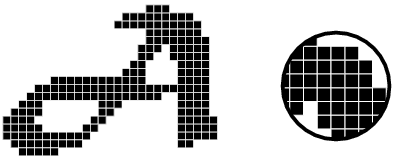
\includegraphics[width=1\linewidth]{trait_images_schema_1b}\\
Une image vectorielle peut être zoomée sans que cela n'altère la qualité du rendu. Ce mode est adapté aux formes et images qui ne sont pas trop complexes : logos, typographie, plans, cartes, etc.  & Pour une image matricielle, le nombre de pixels utilisés par unité de longueur donne un rendu plus ou moins précis des formes de l'image. Un zoom trop important fait apparaître la pixellisation de l'image.\\
\textit{Les formats de fichiers vectoriels sont PostScript, PDF, SVG, etc.}&\textit{ Les formats de fichiers matriciels sont BMP, GIF, PNG, JPEG, etc.}\\
\hline
\end{tabular}
\end{center}

\vspace{0.2cm}
On s'intéresse par la suite au codage des images par le mode matriciel.

\subsection{Notion de calorimétrie}

\begin{center}
{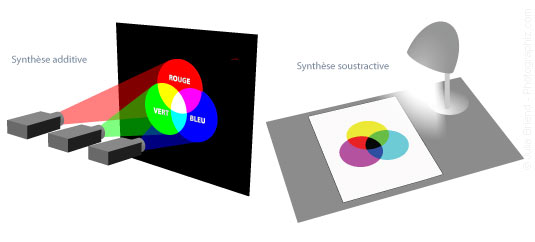
\includegraphics[width=0.7\linewidth]{trait_images_schema_2}}
\end{center}

La \textbf{synthèse additive} est utilisée par les moniteurs et les projecteurs.
Elle est constituée des trois lumières de base qui sont le Rouge, le Vert
et le Bleu (RVB). Les couleurs secondaires sont plus claires
que les primaires, c'est pour cela que leur synthèse est appelée additive.

La \textbf{synthèse soustractive} est utilisée dans l'imprimerie et par
les imprimantes. Les couleurs primaires sont le Cyan, le Magenta,
le Jaune et le Noir (CMJN). Si on mélange deux couleurs primaires, 
le résultat sera une couleur secondaire plus sombre qui absorbera 
donc plus de lumière, c'est pour cette raison que cette synthèse
est nommée soustractive.

Un modèle de colorimétrie est une manière de coder des couleurs
avec des nombres. Nous ne présenterons ici que le modèle RVB
(Rouge Vert Bleu).

Le \textbf{modèle RVB} caractérise une couleur à l'aide de trois paramètres
(chacun sur un octet, soit un nombre de 0 à 255) correspondant
aux trois couleurs Rouge, Vert et Bleu.

\begin{minipage}{3cm}
 \begin{center}
% {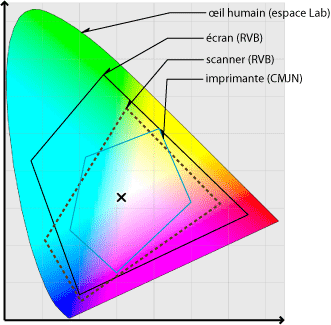
\includegraphics[width=0.4\linewidth]{trait_images_schema_3}}
{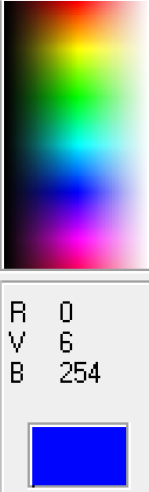
\includegraphics[width=0.4\linewidth]{trait_images_schema_21}}
\end{center}
\end{minipage}
\begin{minipage}{14cm}
 \noindent\fbox{\parbox{\textwidth}{
$\text{00 00 00}_{(16)}$ = (0,0,0) = noir\\
$\text{FF FF FF}_{(16)}$ = (255,255,255) = blanc\\
$\text{FF 00 00}_{(16)}$ = (255,0,0) = rouge\\
}}
\end{minipage}


~~\\

\subsection{Le mode matriciel « bitmap »}

Une matrice de pixels (« picture elements ») est constituée d'un ensemble de points pour former une image. Le pixel représente ainsi le plus petit élément constitutif 
d'une image numérique.

%\noindent\fbox{\parbox{\textwidth}{
%Formats limités à 256 couleurs : GIF, PCX, PGM, etc.\\
%Formats acceptant différentes quantifications BMP, TIFF, TGA, PNG, etc.\\
%Formats limités à 16 millions de couleurs JPEG, etc.
%}}


\begin{minipage}{4cm}
 {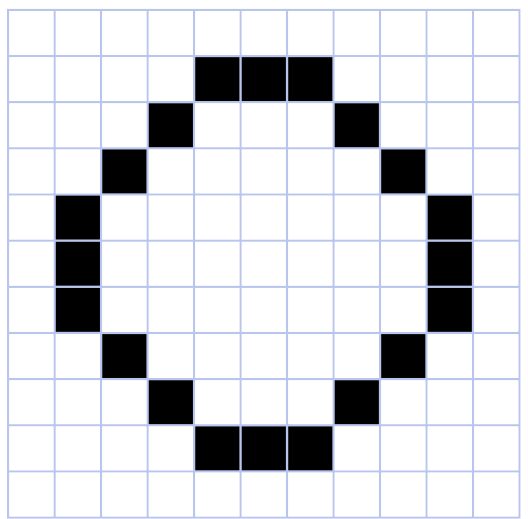
\includegraphics[width=0.5\linewidth]{trait_images_schema_22}}
\end{minipage}
\begin{minipage}{12cm}
La discrétisation d'une image se caractérise par sa \textbf{définition}, c'est-à-dire le nombre de pixels utilisés.
\end{minipage}

~~\\

\begin{minipage}{4cm}
{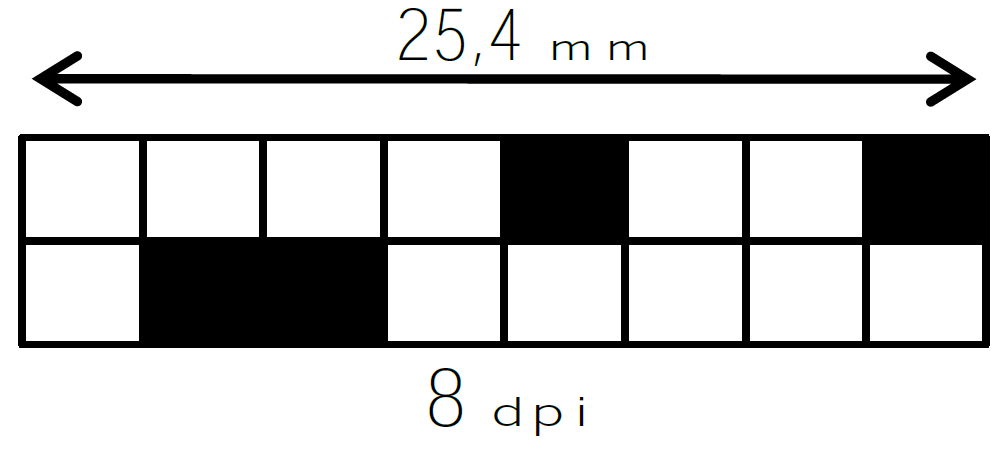
\includegraphics[width=0.9\linewidth]{trait_images_schema_23}}
\end{minipage}
\begin{minipage}{12cm}
 La \textbf{résolution} de l'image établit un lien entre le nombre de pixels d'une image et sa taille réelle. Elle se caractérise par un nombre de pixels par unité de longueur.
\end{minipage}

~~\\

La \textbf{quantification des couleurs} est exprimée en bits par pixel (bpp) :
1 bpp  ( = 1 bit/pixels = deux couleurs : noir et blanc par exemple), 8 bpp (niveaux de gris entre 0 et 255 par exemple,
256 couleurs), etc.

\begin{exemple}
« 800 x 600 » signifie une largeur de 800 et une hauteur de 600 pixels.\\
 « 600 dpi » (« ppp » : point par pouce, « dpi » : dots per inch) 
signifie 600 pixels par pouce (1 pouce = 25,4 mm).
En connaissant le nombre de pixels d'une image et la mémoire 
nécessaire à l'affichage d'un pixel, il est alors possible
de définir exactement la taille qu'occupe le fichier.\\
Une définition du type 800 * 600 avec un codage sur 24 bits 
(3 octets) des couleurs, donne un fichier image de taille
1,44 Mo.\\
\end{exemple}

% La couleur peut être codée directement dans le pixel, ou dans une palette.
% L'organisation d'un fichier bitmap est donnée ci-contre.\\
% \centering{\includegraphics[width=0.4\linewidth]{trait_images_schema_5}}



% 
% \Exem{\textbf{format BMP}\\
% \centering{\includegraphics[angle=90,width=0.8\linewidth]{trait_images_schema_6}}}
% 
% \newpage
% 
% \Exem{\textbf{format BMP}\\
% \centering{\includegraphics[angle=90,width=0.8\linewidth]{trait_images_schema_7}}}
% 
% \newpage

%\newpage
\section{Manipulation des matrices de pixels}
\subsection{Afficher une image à partir d'un fichier  (voir  Activité 1)}

Nous utiliserons la bibliothèque \textbf{image} de matplolib.
\begin{lstlisting}
import matplotlib.pyplot as plt     # import de la bibliothequepyplot (la même que celle utilisée pour l'affichage de courbes)
import matplotlib.image as img     # import de la bibliotheque image

im1=img.imread("image.bmp") # lecture de l'image et stockage dans la variable im1
plt.imshow(im1)  # affichage de l'image
plt.show()

im1.shape     #dimensions de l'image
print (im1)  #affichage du contenu de la varibale im1

\end{lstlisting}
~~\\

\subsection{Créer une image simple (voir Activité 2)}

L'instruction ci-dessous permet de créer une image vide, pour laquelle la couleur de chaque pixel sera codée sur 3 valeurs (RVB par exemple).

\begin{lstlisting}
#Création d'une image vide, avec 3 valeurs par pixels
imV = np.zeros((Ly ,Lx,3))   #Ly est la dimension verticale, Lx la dimension horizontale
\end{lstlisting}

~~\\ Pour modifier la valeur d'un pixel, il suffit de modifier le triplet "RVB" associé au pixel correspondant.
\begin{lstlisting}
p=im2[i,j]   #affecte à la variable p le contenu du pixel situé aux indices i et j

im2[i,j]=[100,50,12]  #affecte au pixel situé aux indices i et j les valeurs R/G/B : 100/50/12
\end{lstlisting}


\section{Transformation d'images}
\subsection{Symétrie d'une image}
cf Activité 4 \\ 
\begin{minipage}{5cm}
 Nous voulons obtenir un effet miroir, c'est à dire
une symétrie par rapport à un axe horizontal.
\begin{center}
{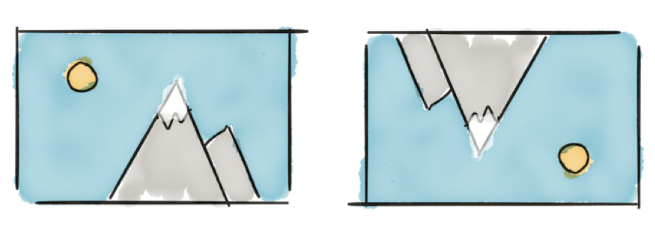
\includegraphics[width=0.9\linewidth]{flip}}
\end{center}
\end{minipage}
\hspace{1cm}
\begin{minipage}{10cm}
 \begin{lstlisting}
def symetrie(im1):
    ''' réalise une symétrie d'axe horizontal '''
    nb_lig,nb_col,nb_comp=im1.shape
    im2=np.zeros((nb_lig,nb_col,nb_comp))
    for i in range(nb_lig):
        for j in range(nb_col):
             im2[i,j]=im1[............]   # compléter cette ligne  % im2[i,j]=im1[nb_lig-i-1,j]   
    return im2
\end{lstlisting}
\end{minipage}



\subsection{Rotation d'une image d'un quart de tour}


cf TP\\ 
\begin{minipage}{5cm}
Nous souhaitons effectuer une rotation de l'image d'un quart de tour dans le sens direct.
\begin{center}
{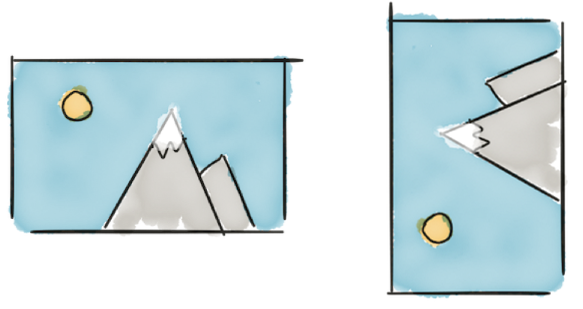
\includegraphics[width=0.9\linewidth]{rot}}
\end{center}
\end{minipage}
\hspace{1cm}
\begin{minipage}{10cm}
 \begin{lstlisting}
def rotation_sens_direct(im1):
    nb_lig,nb_col,nb_comp=im1.shape
    im2=np.zeros(............,..........,nb_coul))   # compléter cette ligne
    for i in range(nb_lig):
        for j in range(nb_col):
             im2[......,.......]=im1[i, j]   # compléter cette ligne
    return im2
\end{lstlisting}
\end{minipage}


%rotation angle quelquonque
%\begin{center}
%{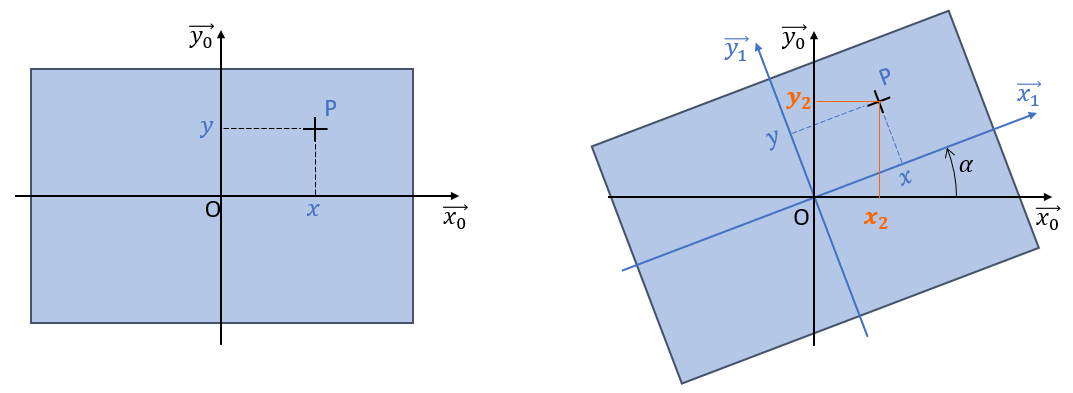
\includegraphics[width=0.9\linewidth]{rotation}}
%\end{center}
%\begin{align}
%\overrightarrow{OP}&=x_2  \vec {x_0}+y_2  \vec{y_0} \notag\\
%&=x \vec {x_1}+y \vec {y_1}\notag\\
%&=x (cos\alpha \vec {x_0}+sin\alpha \vec {y_0})+y (-sin\alpha \vec {x_0}+cos\alpha \vec {y_0}) \notag
%\end{align}
%
%On obtient ainsi les relations permettant le passage des anciennes cordonnées ($x$, $y$) aux nouvelles coordonnées ($x_2$,  $y_2$) :\\
%$\left\{
%\begin{array}{l}
%x_2=xcos\alpha - ysin\alpha\\
%y_2=xsin\alpha + y cos\alpha
%\end{array}
%\right.$


\subsection{Passer en niveau de gris}
\begin{minipage}{6cm}
 Une des possibilités pour obtenir une image en niveau de gris à partir 
d'une image codée sur les 3
composantes de couleur (bleu,vert,rouge) est de remplacer la valeur
de chaque composante de chaque
pixel par la moyenne des valeurs des 3 composantes du pixel considéré.
Cette méthode est simple mais peu convaincante au niveau de l'image.
\end{minipage} \ \ \
\begin{minipage}{11cm}
\begin{lstlisting}
def niveau_gris(matB):
    '''convertit une image rgb en niveau de gris'''
    nb_lig,nb_col,nb_coul=matB.shape
    matC=np.zeros((nb_lig,nb_col))
    for i in range(nb_lig):
        for j in range(nb_col):
            sum=0
            for k in range(nb_coul):
                sum+=matB[i,j,k]
            moy=sum/nb_coul
            matC[i,j]=moy
    return matC  
\end{lstlisting}
\end{minipage}

Pour l'affichage, il faut changer la \textit{Colormap} de \texttt{matplotlib}:
\begin{lstlisting}
plt.imshow ( im  , cmap='gray')                # affichage d'une image en niveau de gris
\end{lstlisting}

\textit{\textbf{Remarque}} : La CIE (Commission Internationale de l'Eclairage) normalise la répartition pour obtenir un niveau de gris correct.
Dans sa norme 709, il est indiqué que pour les images naturelles les poids
respectifs doivent être : 0.2125 * R + 0.7154 * G + 0.0721 * B.


%
%\begin{lstlisting}
%def niveau_gris_norme(matB):
%    nb_lig,nb_col,nb_coul=matB.shape
%    matC=np.zeros((nb_col,nb_lig,nb_coul))
%    for i in range(nb_lig):
%        for j in range(nb_col):
%            gris=int(0.2125*matB[i,j,0]+0.7154*matB[i,j,1]+0.0721*matB[i,j,2])
%            for k in range(nb_coul):
%                matC[j,i,k]=gris
%    return matC
%\end{lstlisting}



\section{Modification par convolution : filtrage}
Le filtrage consiste à appliquer une transformation (appelée filtre) à tout ou partie d'une image numérique en
appliquant un opérateur.

% \begin{itemize}
%  \item Les filtres passe-bas, consistant à atténuer les composantes 
%  de l'image ayant une fréquence haute (pixels
% foncés). Ce type de filtrage est généralement utilisé pour atténuer
% le bruit de l'image, c'est la raison pour
% laquelle on parle habituellement de lissage. Les filtres « moyenneurs »
% sont un type de filtres passe-bas dont
% le principe est de faire la moyenne des valeurs des pixels avoisinants.
% Le résultat de ce filtre est une image
% plus floue.
%   \item Les filtres passe-haut, à l'inverse des passe-bas, atténuent
%   les composantes de basse fréquence de l'image et permettent notamment
%   d'accentuer les détails et le contraste, c'est la raison pour laquelle 
%   le terme de "filtre d'accentuation" est parfois utilisé.
%   
%   \item  Les filtres passe-bande permettant d'obtenir 
%   la différence entre l'image originale et celle obtenue par application
%   d'un filtre passe-bas.
%   \item  Les filtres directionnels appliquant une transformation
%   selon une direction donnée...
%  
% \end{itemize}


Un \textbf{filtre} est une transformation mathématique (appelée produit de convolution)
permettant, pour chaque pixel de la zone à laquelle il s'applique,
de modifier sa valeur en fonction des valeurs des pixels avoisinants,
affectées de coefficients.\\
\begin{center}
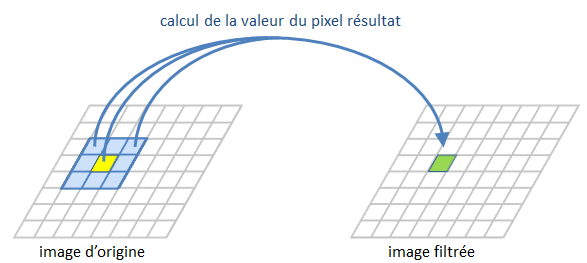
\includegraphics[width=0.8\linewidth]{filtrage}
\end{center}

Le filtre est représenté par un tableau (matrice), caractérisé par
ses dimensions et ses coefficients, dont le centre correspond au pixel 
concerné. Les coefficients du tableau déterminent les propriétés du filtre.


\begin{exemple}
Prenons le cas d'une matrice 3x3, donc un tableau de neuf nombres
représentés
ici par a, b, c, ..., i qui sont les paramètres du filtre et que l'on
peut donc définir (cf. figure).
~~\\

L'image est en niveau de gris (256 valeurs), le pixel considéré a un niveau de gris
égal à 115.
~~\\

La valeur 115 est remplacée par la somme de 9 produits : 

45.a + 60.b + 81.c + 82.d + 115.e + 133.f + 130.g + 154.h + 147.i

Afin de normaliser ce résultat, bien souvent, on divisera ce résultat
par la somme des coefficients du filtre, soit a+b+c+d+e+f+g+h+i.
\end{exemple}

\begin{center}
{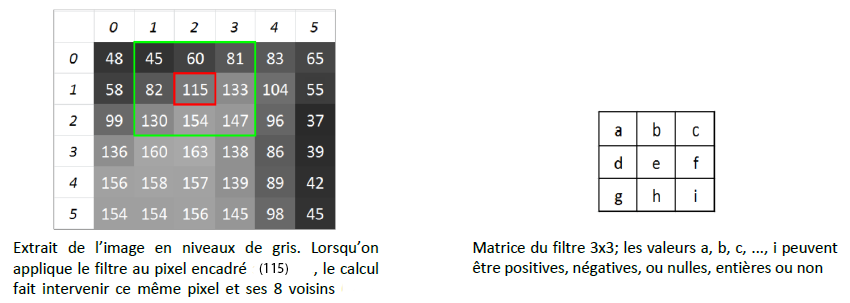
\includegraphics[width=1\linewidth]{trait_images_schema_11}}
\end{center}

\textit{\textbf{Remarque :} Qu'en est-il pour un pixel appartenant à la bordure de l'image,
car il n'a pas tous ses voisins ?\\
La solution la plus simple est d'ignorer ces pixels : on balaye l'image de la deuxième ligne à l'avant-dernière, et pour chaque 
ligne, de la deuxième colonne à l'avant-dernière. \\ Des solutions plus évoluées utilisent aussi des matrices particulières pour les bords.}
%~~\\
%
%Que se passe-t-il si le résultat du calcul sort de l'intervalle [0;255]
%correspondant aux valeurs extrêmes des composantes RVB ?
%\begin{itemize}
% \item Solution 1 : le résultat (différent pour chaque pixel) est divisé 
% par la somme des coefficients du filtre.
% \item Solution 2 : On écrête tout résultat supérieur à 255 ou inférieur à 0
% \item Solution 3 : On ramène l'ensemble des résultats dans 
% l'intervalle [0,255] en appliquant une proportionnalité. Cela nécessite 
% de faire une recherche de la valeur min et de la valeur max dans toute
% l'image.
\begin{center}
{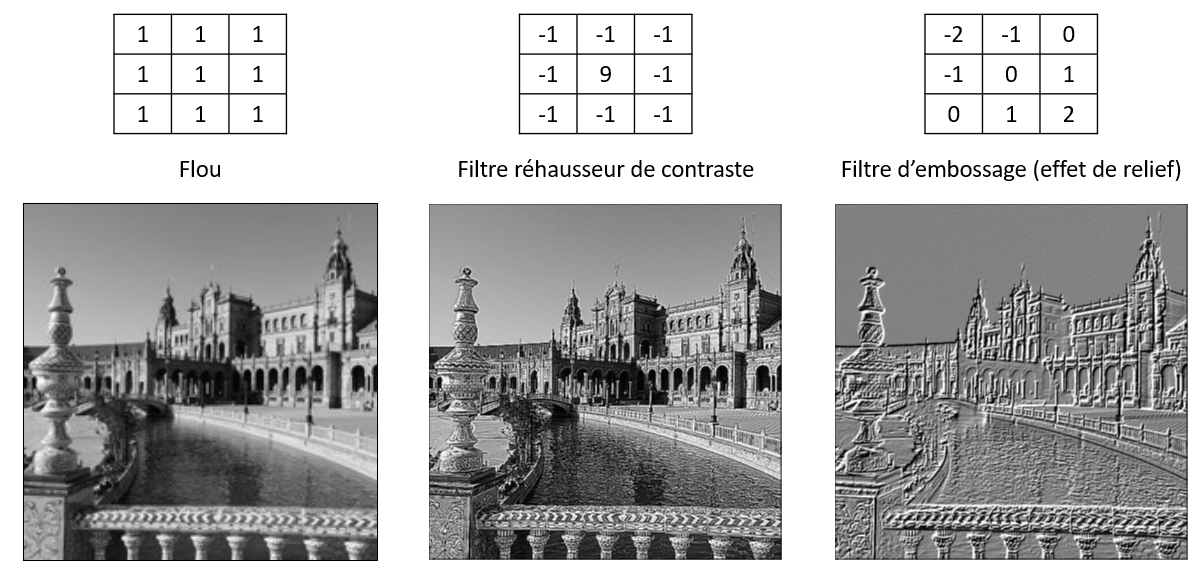
\includegraphics[width=1\linewidth]{filtres2}}
\end{center}
%\end{itemize}

 \vspace{5cm}Sources:\\
- UPSTI 
\includegraphics[width=0.1 \linewidth]{logo_upsti} 
 
% 
% \section{Programmation graphique d'un jeu de rugby}
% 
% \subsection{Conception d'une application sportive }
% 
% L'application « Rugby Manager » est un
% jeu destiné aux smartphones et aux tablettes. Il
% permet de créer une équipe, de l'entraîner et de
% jouer avec elle. Il est possible de joueur seul (contre
% l'intelligence artificielle du logiciel) ou en mode multijoueurs.
% Enfin, l'application est utilisable en ligne ou
% en Bluetooth.
% 
% 
% 
% L'objectif aujourd'hui est de programmer un certain nombre de fonction qui seront utilisées pour créer cette application.
% 
% \subsection*{Partie graphique du mode jeu}
% Dans cette partie nous souhaitons tout d'abord représenter la partie graphique du mode jeu, c'est-à-dire :
% 
% \begin{itemize}
%  \item un terrain ;
%  \item deux équipes ;
%  \item un ballon.
% \end{itemize}
% 
% nous allons réaliser une étude partielle de ces fonctionnalités.
% 
% On souhaite afficher l'image du terrain de rugby suivant,
% enregistrée
% dans le répertoire "C: CCP" 
% sous le nom \textit{stade.bmp}:
% 
% \begin{center}
% \includegraphics[width=.5\textwidth]{stade.png}
% \end{center}
% 
% ~~\\
% 
% \noindent\fbox{\parbox{\textwidth}{
% \textbf{Objectif}~~\\
% 
% Les compétences évaluées dans ce TP portent sur le traitement des images.
% Il s'agit d'utiliser la bibliothèque d'image décrite en annexe pour compléter ou modifier des fonctions d'affichages 
% de l'image du terrain et des pixels des maillots des joueurs.
% Dans un second temps il s'agit de mettre en place un "floutage" d'une image pour la mettre en arrière plan dans le mode statistique.
% }}
% % 
% % \begin{objectif}
% % Les compétences évaluées dans cette partie portent sur le traitement des images.
% % Il s'agit d'utiliser la bibliothèque d'image décrite en annexe pour compléter ou modifier des fonctions d'affichages 
% % de l'image du terrain et des pixels des maillots des joueurs.
% % \end{objectif}
% 
% \Q{ Créer un programme qui permet:}
% \begin{itemize}
%  \item de se placer dans le dossier où se trouve l'image ;
%   \item d'ouvrir l'image et de la stocker dans une variable \textit{image\_terrain} ;
%   \item d'afficher l'image en arrière plan.
% \end{itemize}
% 
% il est nécessaire ensuite nécessaire de connaître les dimensions de l'image qui peut être connu grâce aux deux fonctions suivantes
% \begin{lstlisting}
% xmax= picture.shape[1]    #taille du tableau 
% ymax= picture.shape[0]   #taille du tableau
% print ("taille de l'image : %d x %d" % (xmax,ymax))
% \end{lstlisting}
% 
% Pour obtenir la couleur du pixel il  suffit donc de choisir le ou les bons indices du tableau.
% ~~\\
% 
% \Q{Donner les instructions qui permettent de faire cette opération 
% et de stocker le résultat dans deux variables \textit{dim\_long} et \textit{dim\_larg} respectivement 
% dimension en longueur et en largeur.
% Afficher ensuite le résultat sous la forme ("longueur x largeur").}
% ~~\\
% 
% On propose dans un premier temps de représenter les joueurs par 4 pixels disposés en carré ayant la couleur du maillot de l'équipe. 
% Le choix des couleurs de maillots doit être laissé libre à l'utilisateur. Cependant, le vert correspondant à la couleur du terrain
% et le blanc correspondant à la couleur du ballon et des lignes ne pourront pas être utilisés.
% ~~\\
% Précisons que les lignes font 2 pixels de large, sur une image qui en fait 620, et qu'il est facile de se positionner au
% centre du terrain. Les lignes pointillées des 40 sont elles à 50 pixels du centre.
% ~~\\
% 
% \Q{Créer une fonction \textit{coul()} qui permet de connaître la couleur exacte du terrain et de la stocker dans une variable \textit{coul\_ter}.
% L'argument d'entrée de la fonction est la variable  \textit{image}, la sortie est la variable \textit{coul\_ter}. Attention : on choisira comme pixel de référence un des pixels le plus proche du centre du terrain.}
% ~~\\
% 
% \Q{Quel est le type de la variable \textit{coul\_ter}.\\
% Sur combien de bits mémoire est codé un pixel ?}
% ~~\\
% % 
% % \Q{Créer une fonction \textit{maillot()} qui utilise 
% % la fonction précédente et qui renvoie la liste des couleurs interdites pour les maillots.}
% 
% \subsection*{Partie graphique du mode statistiques}
% 
% \subsubsection{Floutage de l'image}
% \fbox{\parbox{\textwidth}{
% \textbf{Objectif}~~\\
% Dans cette partie, nous intéressons d'abord au traitement d'image évolué : la mise en place un "floutage"
% d'une image pour l'arrière plan du mode statistique. Nous étudierons par la suite des fonctions simples de statistiques qui permettent d'alimenter ce mode du jeu.
% }}
% 
% On s'intéresse donc ici à un autre mode du jeu vidéo : le mode statistique. Dans ce mode, une image
% de jeu floue va être mise en arrière plan. Nous allons donc étudier les fonctions permettant d'effectuer ce floutage.
% ~~\\
% Pour réaliser un floutage par moyenne simple sur la matrice de pixels, il faut lui appliquer un filtre, que l'on appelle également un masque.
% Afin de bien comprendre ce principe, nous proposons d'étudier un exemple de filtrage :
% On considère les matrices  %$A=((1/9&1/9&1/9@1/9&1/9&1/9@1/9&1/9&1/9))$ et $B=(?(?(5&6&7@-5&-6&-7@1&1&1)     ?(8&9&10@-8&-9&-10@1&1&1)@?(2   &2   &3)      ?( 3     &4  &  4)@?(0   &0   &1)      ?( 2     &3  &  3)))$
% 
%  \begin{equation*}
% A=\left(             
% {\begin{array}{ccc}
%    1/9 & 1/9 & 1/9 \\
%   1/9 & 1/9 & 1/9 \\
%      1/9 & 1/9 & 1/9
%    \end{array} }
%   \right)
% \end{equation*}
% 
% et
% 
% \begin{equation*}
% B=\left(             
% {\begin{array}{cccccc}
%    5 & 6 & 7 & 8 & 9& 10 \\
%     - \ 5 & - \  6 & - \  7 & -  \ 8 & - \  9& -  \ 10 \\
%     1 & 1 & 1 & 1 & 1 & 1\\
%      2 & 2 & 3 & 3 & 4 & 4\\
%       0 & 0 & 1 & 3 & 3 & 3
%    \end{array} }
%   \right) \ .
% \end{equation*}
% 
% 
% Pour chaque élément \textit{bij} de B, on considère la matrice 3×3 \textit{Bij} qui l'entoure, on calcule le produit de convolution de A par \textit{Bij} \textbf{(multiplication classique \textit{A*Bij})} et on note \textit{cij} la somme des coefficients de la matrice produit obtenue (on pourra utiliser la fonction \textit{np.sum} sur une liste). 
% ~~\\
% Si \textit{bij} est un élément en bordure de B, on posera \textit{cij = bij}. On forme ainsi une nouvelle matrice C dont les éléments intérieurs sont les \textit{cij} (et les éléments au bord sont les \textit{bij}).
% 
% 
% \begin{center}
% 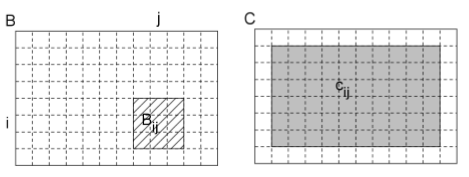
\includegraphics[width=.5\textwidth]{filtre.png}
% \end{center}
% 
% 
% On dit qu'on a filtré la matrice B par la matrice A, ou qu'on a appliqué le masque (filtre) A sur l'image B. 
% ~~\\
% \Q{Compléter la fonction \textit{filtrer1(filtreA,matB)} qui prend en argument une matrice carrée \textit{filtreA} de dimension \textit{taille×taille} (taille est un entier impaire $?$ 3) et une matrice quelconque \textit{matB} de dimensions supérieures, et qui renvoie la matrice C. On remarquera que si $taille>3$, la bordure devra être plus épaisse. Vous pouvez utiliser les fonctions du module numpy que vous jugez judicieuses sans préciser l'importation.}
% 
% ~~\\
% 
% On souhaite maintenant appliquer le filtre A à une matrice de pixels B, c'est à dire aux 3 tableaux B[:,:,0], B[:,:,1], B[:,:,2] et enregistrer le résultat dans une matrice C de même format que B. 
% 
% ~~\\
% \Q{Créer une fonction \textit{filtrer(filtreA,matB)} qui prend en argument une matrice carrée \textit{filtreA} de dimension \textit{taille×taille} et un tableau numpy\textit{ matB} de dimensions $n×p×3$,et qui renvoie le tableau C de dimensions  identiques. 
% Vous pourrez calculer successivement C[:,:,0], C[:,:,1], C[:,:,2] à l'aide d'une boucle.}
% 
% ~~\\
% Ces matrices réalisent un floutage par moyenne simple (coefficients tous égaux, de somme 1). Plus la taille du filtre est grande, plus le flou sera fort. On peut améliorer cette technique en utilisant un flou gaussien. Son principe est de calculer une moyenne pondérée en accordant plus de poids au pixel central et en diminuant le poids des pixels périphériques. 
% ~~\\
% La matrice servant de filtre est calculée selon le modèle d'une courbe de Gauss (courbe en cloche) à 2 dimensions : 
% ~~\\
% La fonction de Laplace-Gauss est $G(x)=\frac{1}{\sigma \sqrt{2\pi}} e^{-\frac{x^2}{2\sigma ^2}}$.
% A deux dimensions on utilise $G(x,y)=\frac{1}{\sigma \sqrt{2\pi}} e^{-\frac{x^2+y^2}{2\sigma ^2}}$.
% ~~\\
% Plus l'écart type $\sigma$ est grand, plus l'image sera floutée. En pratique, $\sigma$ et la taille (impaire) du filtre étant fixés, on calcule chaque élément de la matrice filtre par la formule $(x,y)=k.e^{-\frac{x^2+y^2}{2\sigma ^2}}$ , 
% \begin{itemize}
% \item où $x$ et $y$ sont le nombre de lignes et de colonnes qui séparent cet élément du centre,
% \item et $k$ un coefficient constant tel que la somme de tous les éléments (de type float) ainsi calculés soit 1.
% \end{itemize}
%  ~~\\ 
% Par exemple, pour \textit{taille=5} et $\sigma=0.9$, le filtre est proche de : %$ 1/1002 (?(?(1&9&17@9&58&107@17&107&198)     ?(9@58@107  )?(1@9@17)@?(9  &58  &107)       ?(58&9)@?(1   &9   &17)?(          9&1)))$
% ~~\\
% \Q{Écrire la fonction la fonction \textit{matriceFlouGaussien(taille,sigma)} qui prend en argument la \textit{taille} (impaire) de la matrice de floutage, \textit{sigma} l'écart type de déviation standard et qui retourne la matrice filtre correspondant au niveau gaussien. Encore une fois, vous pouvez utiliser les fonctions du module numpy que vous jugez judicieuses sans préciser l'importation.} 
% 
% 
% ~~\\
% \Q{Écrire ensuite la fonction \textit{FloutageGaussien(tabPix,taille,sigma)} qui utilise la fonction \textit{matriceFlouGaussien(taille,sigma)} et \textit{filtrer(filtreA,matB)}  et qui renvoie la matrice \textit{tabPix} qui a été floutée grâce au filtre défini dans la fonction \textit{matriceFlouGaussien}.}
% 
% 
% \subsubsection{Détection d'un joueur}
% 
% \fbox{\parbox{\textwidth}{
% \textbf{Objectif}~~\\
% Dans cette partie, nous intéressons d'abord au traitement d'image évolué : la rotation de l'image et la détection de joueur sur l'image.
% }}
% ~~\\
% 
% \Q{Écrire la fonction qui permet de faire une rotation de $-\pi/2$ de notre image.}
% 
% 
% Pour permettre la détection d'un joueur sur le terrain, il faut définir les contours principaux des objets présents sur le terrain.
% 
% ~~\\
% 
% \Q{Écrire la fonction qui permet de passer en niveau de gris notre image}
% 
% 
% ~~\\
% 
% \Q{Écrire la fonction qui permet de définir les contours.}


\label{LastPage}
